% !TeX encoding = UTF-8
% !TeX program = xelatex
% !TeX spellcheck = fr_CA
\documentclass[nuit,charter,pied]{BeamerJS}
\title{Variables aléatoires discrètes}
\subtitle{À l'intention des étudiants de STT-1500}
\institute{Université Laval}
\fonction{Département de mathématiques et de statistique}
\logotitre{../logo_UL.pdf}
\author{Jérôme Soucy}
\date{Hiver 2025}

\usepackage{adjustbox}
\usepackage{xstring}
\usepackage{commandesJS}
\addbibresource{../references.bib}
\NouvelleBoiteJS{rems}{Remarques}{Accent}{AccentBG}
\usepackage{calc}
\usepackage{nicefrac}
\usetikzlibrary{calc}
\usepackage{array}
\usepackage{booktabs}
\usepackage{relsize}

\pgfplotsset{
    every axis/.append style={
        /pgfplots/tick label style={/pgf/number format/use comma}
    }
}
\begin{document}
\begin{frame}[plain,noframenumbering]
	\titlepage
\end{frame}

\begin{frame}{Résumé}
\tableofcontents
\end{frame}
\section{Variables aléatoires}
\begin{frame}{Définition}
	\begin{defn}{}
		Une \defi{variable aléatoire} est une quantité dont la valeur numérique dépend du résultat d'une expérience aléatoire.
	\end{defn}\pause
	\begin{rems}
	\begin{enumerate}
		\item On écrit souvent v.a. pour signifier variable aléatoire.\\ \pause
		\item On utilise généralement les lettres majuscules du début de l'alphabet pour dénoter des événements, alors que les lettres majuscules près de la fin de l'alphabet désignent des variables aléatoires.\\ \pause
		\item Si $\omega$ est le résultat de l'expérience aléatoire, on note $X(\omega)$ la valeur de la variable aléatoire $X$.
	\end{enumerate}
	\end{rems}
\end{frame}

\begin{frame}{Début d'un exemple}
	Soit $\mathcal{E}$ l'expérience aléatoire consistant à lancer une pièce de monnaie trois fois et de noter si elle tombe sur pile ($P$) ou face ($F$). L'espace fondamental de $\mathcal{E}$ est:
		\[\mathlarger{{\scriptstyle\Omega=\{(P,P,P),(P,P,F),(P,F,P),(F,P,P),(F,F,P),(F,P,F),(P,F,F),(F,F,F)\}}.}\]
		\pause
	On peut définir $X$ comme étant le nombre d'apparition(s) de pile parmi les trois lancers.
	\pause
	\begin{itemize}
		\item Les valeurs que $X$ peut prendre sont $0,1,2$ et $3$.
		\item Par exemple, $X\left((P,P,F)\right)=2$.
	\end{itemize}
\end{frame}
\begin{frame}{Distribution d'une variable aléatoire}
	Étant donné un sous-ensemble $B$ de $\R$, on peut s'intéresser à la probabilité qu'une variable aléatoire $X$ prenne ses valeurs dans $B$.\pause
	\begin{defn}{}
		Soit $X$ une variable aléatoire. La \defi{distribution} de $X$ est une fonction qui associe aux sous-ensembles $B$ de $\R$ le nombre
		\[\P{\omega\in\Omega:X(\omega)\in B}.\]
	\end{defn}\pause
\begin{rem}
	On préfère généralement écrire $\P{X \in B}$ plutôt que $\P{X^{-1}(B)}$ ou $\P{\omega \in \Omega : X(\omega) \in B}$, afin de simplifier la notation et de privilégier une forme plus compacte et intuitive.
\end{rem}
\end{frame}

\begin{frame}{Distributions discrètes}
	\begin{defn}{}
		Une variable aléatoire $X$ est dite \defi{discrète} si sa distribution est discrète, c'est-à-dire si sa distribution est de la forme
		\[\P{X\in B}=\sum_{x\in B}p(x)\]
		pour une certaine fonction $p(x)$.
	\end{defn}
	\pause
	\begin{rem}
	La fonction $p(x)$, parfois notée $p_X(x)$, s'appelle alors la \defi{fonction de masse} de la variable aléatoire $X$. On peut aussi l'appeler \defi{fonction de probabilité} ou \defi{fonction de masse de probabilité}.
	\end{rem}
\end{frame}
%\begin{frame}{Une image}
%	\vspace{-1cm}
%	\begin{center}
%	\begin{tikzpicture}
%
%        % Définition des ensembles
%        \draw(-6,-2)--(-6,2)--(-1.2,2)--(-1.2,-2) -- cycle;
%        \draw[line width=1pt] (-3,0) ellipse (2 and 1.5);
%        \draw[line width=1pt] (3,0) ellipse (2 and 1.5);
%        \draw (-3.5,2)node[above]{$\Omega$};
%       % Noms des ensembles
%        \node[above] at (-3,1.7) {\large $X^{-1}(B)$};
%        \node at (3,1.7) {\large $B$};
%        
%        \node at (-3,-0.3) {\large $\omega$};
%        \node at (3,-0.3) {\large $x$};
%
%        % Points
%        \fill (-3,-0.3) circle (2pt);
%        \fill (3,-0.3) circle (2pt);
%
%        % Fonction X
%        \draw[->, line width=1pt] (-3,-0.3) to[out=30,in=150] node[above] {\large $X$} (3,-0.3);
%
%    \end{tikzpicture}
%	%	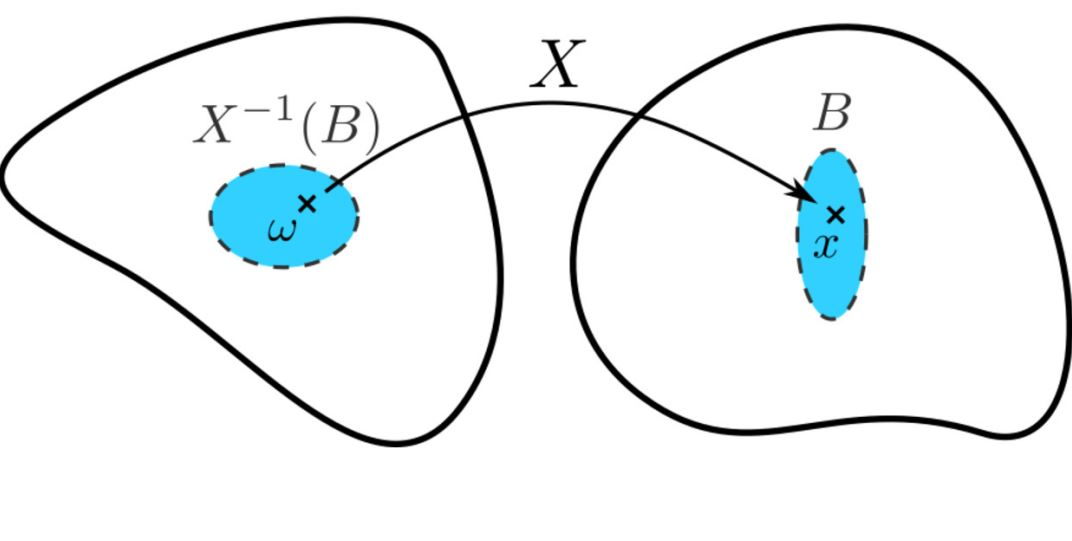
\includegraphics[width=10cm]{images/va.jpg}\\
%	%	Image provenant de \cite{wiki:Variable_aleatoire}
%	\end{center}
%\end{frame}
\begin{frame}{Exemple (suite)}
	Rappelons que $X$ est le nombre d'apparition(s) de pile parmi les trois lancers.\pause
	
	On constate que
	\begin{align*}
		\P{X=0}&=\frac{1}{8},\\
		\P{X=1}&=\frac{3}{8},\\
		\P{X=2}&=\frac{3}{8},\\
		\P{X=3}&=\frac{1}{8}.
	\end{align*}\pause
	Pour des nombres $k$ à l'extérieur de l'ensemble $\{0,1,2,3\}$, nous avons que $\P{X=k}=0$.
\end{frame}
\begin{frame}{Une représentation graphique}
	\hfill
	\begin{minipage}[c]{.4\textwidth}
		\begin{tikzpicture}
			\draw[thick] (-1,0) -- (4,0);
			\draw[thick] (0,0) node[below]{$0$} -- (0,1) node[above]{$\frac{1}{8}$};
			\draw[thick] (1,0) node[below]{$1$} -- (1,3) node[above]{$\frac{3}{8}$};
			\draw[thick] (2,0) node[below]{$2$} -- (2,3) node[above]{$\frac{3}{8}$};
			\draw[thick] (3,0) node[below]{$3$} -- (3,1) node[above]{$\frac{1}{8}$};
		\end{tikzpicture}
	\end{minipage} 
	\hfill
	\begin{minipage}[c]{.4\textwidth}
		\begin{displaymath}
			\P{X=k}=\begin{cases}
				\frac{1}{8} &\text{si $k\in\{0,3\}$},\\
				\frac{3}{8} &\text{si $k\in\{1,2\}$},\\
				0 &\text{sinon}.
				\end{cases}
		\end{displaymath}
	\end{minipage}
	\hfill
\end{frame}
\begin{frame}{Une représentation graphique}
	\hfill
	\begin{minipage}[c]{.35\textwidth}
		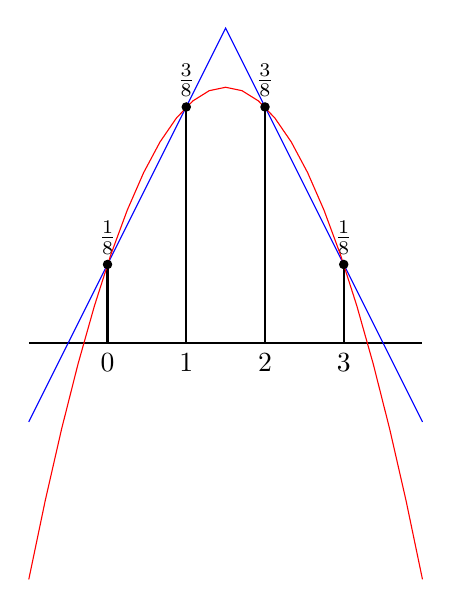
\begin{tikzpicture}[domain=-1:4]
			\draw[thick] (-1,0) -- (4,0);
			\draw[thick] (0,0) node[below]{$0$} -- (0,1) node[above]{$\frac{1}{8}$};
			\draw[thick] (1,0) node[below]{$1$} -- (1,3) node[above]{$\frac{3}{8}$};
			\draw[thick] (2,0) node[below]{$2$} -- (2,3) node[above]{$\frac{3}{8}$};
			\draw[thick] (3,0) node[below]{$3$} -- (3,1) node[above]{$\frac{1}{8}$};
			\draw[color=blue]    plot (\x,{4-abs(2*\x-3)});
			\draw[color=red]    plot (\x,{8*(-0.125*\x*\x+0.375*\x+0.125)});
			\draw[fill=black] (0,1) circle (1.5pt);
			\draw[fill=black] (1,3) circle (1.5pt);
			\draw[fill=black] (2,3) circle (1.5pt);
			\draw[fill=black] (3,1) circle (1.5pt);
		\end{tikzpicture}
	\end{minipage}
	\hfill
	\begin{minipage}[c]{.6\textwidth}
		\begin{flushleft}
			Si la fonction de masse d'une variable aléatoire caractérise celle-ci, on peut décrire cette même fonction de plusieurs manières.
		\end{flushleft}
	\vfill
		{\color{blue}
		\begin{displaymath}
			\P{X=k}=\begin{cases}
				\frac{4-|2k-3|}{8} &\text{si $k\in\{0,1,2,3\}$},\\
				0 &\text{sinon}.
			\end{cases}
		\end{displaymath}
		}
		{\color{red}
			\begin{displaymath}
				\P{X=k}=\begin{cases}
					\frac{-k^2+3k+1}{8} &\text{si $k\in\{0,1,2,3\}$},\\
					0 &\text{sinon}.
				\end{cases}
			\end{displaymath}
		}
	\vfill
	\end{minipage}
	\hfill
\end{frame}
\begin{frame}{Propriétés de la fonction de masse}
	\begin{prop}
		Soit $X$ est une v.a. de fonction de masse $p(x)$. Alors
		\begin{align}
			p(x)&\geq 0~\forall x\in\R\,;\\ 
			\sum_{x\in\R}p(x)&=1.
		\end{align}
		De plus, $p(x)>0$ pour un nombre fini ou infini dénombrable de $x$.
	\end{prop}
\end{frame}
\begin{frame}{Propriétés de la fonction de masse}
	\begin{rem}
		Si une fonction $p:\R\rightarrow \R$ vérifie les équations (1) et (2) ci-dessous,
		\begin{align}
			p(x)&\geq 0~\forall x\in\R\,;\\ 
			\sum_{x\in\R}p(x)&=1,
		\end{align}
		on peut concevoir une expérience aléatoire $\mathcal{E}$, et définir une v.a. $X$ qui découle de $\mathcal{E}$, dont la fonction de masse est $p(x)$. C'est pourquoi toute fonction satisfaisant (1) et (2) s'appelle une fonction de masse sur $\R$.
	\end{rem}
\end{frame}

\section{Espérance d'une v.a. discrète}

\begin{frame}{Définition}
	\begin{defn}
		Soit $X$ une v.a. discrète de fonction dont la fonction de masse est $p(x)$ et qui vérifie
		\[\sum_{x\in\R}|x|\,p(x)<\infty.\]
		\defi{L'espérance mathématique} de $X$ est définie par
		\[\Es{X}=\sum_{x\in\R}xp(x).\]
	\end{defn}
	\end{frame}
\begin{frame}{Une remarque sur la définition de l'espérance}
	\begin{rem}
		La condition \[\sum_{x\in\R}|x|\,p(x)<\infty\] est présente pour s'assurer que l'espérance existe. Nous verrons quelques variables aléatoires pour lesquelles l'espérance n'est pas définie. Je vous invite à lire la section 4.7 des notes de cours afin de rencontrer quelques cas problématiques.
	\end{rem}
\end{frame}
\begin{frame}{L'espérance de \(X\) dans notre exemple}
Nous avons que
\begin{align*}
	\Es{X}&=\sum_{x\in\R}xp(x)&\text{(par définition)}\\
	&\sum_{x\in\{0,1,2,3\}}xp(x)&\text{car $p(x)=0$ si $x\notin\{0,1,2,3\}$}\\
	&=0\cdot p(0)+1\cdot p(1)+2\cdot p(2)+3\cdot p(3)\\
	&=0\cdot \frac{1}{8}+1\cdot \frac{3}{8}+2\cdot \frac{3}{8}+3\cdot \frac{1}{8}\\
	&=\frac{3}{2}.
\end{align*}

\end{frame}
\section{Quelques distributions discrètes}

\begin{frame}{La loi de Bernoulli}
	
	\begin{defn}
		Une \defi{épreuve de Bernoulli} est une expérience aléatoire avec deux résultats possibles, que l'on nomme \textit{succès} et \textit{échec}.
	\end{defn}\pause
	\begin{defn}
		On réalise une épreuve de Bernoulli. La v.a. $X$ prend la valeur $1$ si le résultat de l'expérience est un succès, et la valeur $0$ s'il s'agit d'un échec. Si $p$ désigne la probabilité de succès, on dira que $X$ est une v.a. dont la distribution de probabilité est la \defi{loi de Bernoulli de paramètre $p$}. On écrira
		\[X\sim \loiBernoulli{p}.\]
	\end{defn}
\end{frame}
\begin{frame}{Exemple d'un v.a. ayant une distribution de Bernoulli}
	On lance un dé à $6$ faces régulier. L'expérience est qualifiée de succès si c'est la face $6$ qui est obtenue.\pause~ On définit la variable aléatoire $X$ de telle sorte que $X=1$ si la face $6$ est obtenue et $X=0$ dans le cas contraire.~\pause Ainsi :
	\begin{displaymath}
		\P{X=k}=\begin{cases}
			\frac{1}{6} &\text{si $k=1$},\\
			\frac{5}{6} &\text{si $k=0$},\\
			0 &\text{sinon}.
		\end{cases}
	\end{displaymath}\pause
Nous avons que $X\sim \loiBernoulli{\frac{1}{6}}$.\pause~ Son espérance est $\Es{X}=1\cdot\frac{1}{6}+0\cdot\frac{5}{6}=\frac{1}{6}$.\pause~ En général, l'espérance d'une v.a. dont la loi a comme loi une distribution de Bernoulli de paramètre $p$ est $p$. Cette loi est d'une grande simplicité. Elle est souvent utilisée pour décomposer des lois plus complexes en éléments plus simples.
\end{frame}	
\begin{frame}{La loi binomiale}
	
	\begin{defn}
		On réalise $n$ répétitions d'une même épreuve de Bernoulli de paramètre $p$. On définit la variable $X$ comme étant le nombre de succès observés lors de ces $n$ épreuves. On dira alors que $X$ est une v.a. dont la distribution de probabilité est la \defi{loi binomiale de paramètres $n$ et $p$}. On écrira
		\[X\sim \loibinomiale{n}{p}.\]
	\end{defn}
\end{frame}
\begin{frame}{Fonction de masse d'une v.a. de loi binomiale}
	\begin{defn}
		La fonction de masse d'une v.a. $X$ dont la distribution de probabilité est une loi binomiale de paramètres $n$ et $p$ est donnée par
		\[
		\P{X=k}=\begin{cases} \binom{n}{k}p^k(1-p)^{n-k} &\text{si}~k\in\{0,1,2,\ldots,n\},\\
			0 & \text{sinon}
			.\end{cases}
		\]
	\end{defn}
\end{frame}
\begin{frame}{Exemple d'un v.a. ayant une distribution binomiale}
	On lance un dé à $6$ faces régulier $10$ fois. Chaque lancer est un succès si c'est la face $1$ qui est obtenue et un échec sinon. La variable aléatoire $X$ correspond au nombre de succès lors de ces $10$ lancers. Pour des valeurs entières de $k$ entre $0$ et $10$, on constate qu'il y a $\binom{10}{k}$ manières d'obtenir $k$ succès (et $10-k$ échecs) lors de ces $10$ lancers.\pause
	\begin{displaymath}
		\P{X=k}=\begin{cases}
			\binom{10}{k}\frac{5^{10-k}}{6^{10}} &\text{si $k\in\{0,1,2,\ldots,n\}$},\\
			0 &\text{sinon}.
		\end{cases}
	\end{displaymath}\pause
	\textbf{Calcul de l'espérance}\\
	\[\Es{X}=1\cdot\binom{10}{1}\frac{5^{9}}{6^{10}}+2\cdot\binom{10}{2}\frac{5^{8}}{6^{10}}+\ldots+10\cdot\binom{10}{10}\frac{5^{0}}{6^{10}}=\frac{5}{3}=10\cdot\frac{1}{6}.\]
\end{frame}
\begin{frame}{L'usine de bonbons}
	Imaginons une usine qui fabrique des bonbons. Elle en fabrique \num{10000} par jour. Chaque bonbon a une probabilité $\num{0,001}$ d'être rejeté au contrôle de la qualité. Quelle est la probabilité que pour une journée donnée, le contrôle de la qualité rejette 4 bonbons ou moins?\pause
	
	Soit $X$ la variable aléatoire correspondant au nombre de bonbons rejetés lors d'une journée. $X\sim\loibinomiale[num]{\num{10000}}{\num{0,001}}$. On doit calculer
	\[\sum_{k=0}^4\binom{\num{10000}}{k}(\num{0,001})^k(\num{0,999})^{\num{10000}-k}\approx \num{0,02919595}.\]
\end{frame}
\begin{frame}[t]{Fonction de masse?}
	Il faut vérifier que 
		\[
	\P{X=k}=\begin{cases} \binom{n}{k}p^k(1-p)^{n-k} &\text{si}~k\in\{0,1,2,\ldots,n\},\\
		0 & \text{sinon}
		,\end{cases}
	\]
	est une fonction de masse.
\end{frame}
\begin{frame}[t]{L'espérance d'une binomiale}
	\begin{thm}{}
		L'espérance d'une v.a. suivant une loi binomiale de paramètre $n$ et $p$ est $np$.
	\end{thm}\pause
	\begin{rem}{} Nous pouvons démonter ce résultat directement avec la définition de l'espérance, ou encore observer qu'une variable aléatoire dont la loi est une binomiale de paramètre $n$ et $p$ peut s'écrire comme une somme de $n$ variables aléatoires dont la distribution suit une loi de Bernoulli de paramètre $p$. Il nous faut alors utiliser la propriété de l'espérance voulant que l'espérance d'une somme corresponde à la somme des espérances.
	\end{rem}
\end{frame}
\begin{frame}{La loi géométrique}
	
	\begin{defn}
		On réalise une suite d'épreuves de Bernoulli de paramètre $p$. On définit la variable $X$ comme étant le nombre d'étapes nécessaires avant d'observer le premier succès. On dira que $X$ est une v.a. dont la distribution de probabilité est la \defi{loi géométrique de paramètre $p$}, et on écrira
		\[X\sim \loigeometrique{p}.\]
	\end{defn}
	\end{frame}
	\begin{frame}{Fonction de masse d'une v.a. de loi géométrique}
	\begin{prop}
		La fonction de masse d'une v.a. $X$ dont la distribution de probabilité est une loi géométrique de paramètre $p$ est donnée par
		\[
		\P{X=k}=\begin{cases} (1-p)^{k-1}p &\text{si}~k\in\{1,2,3\ldots\},\\
			0 & \text{sinon}
			.\end{cases}
		\]
	\end{prop}
\end{frame}
\begin{frame}[t]{Exemple d'une v.a. ayant la loi géométrique comme distribution}
	On lance un dé régulier à $6$ faces jusqu'à l'obtention de la face $1$. On note $X$ le nombre de lancers nécessaires pour réaliser cet événement. La variable $X$ suit une loi géométrique de paramètre $\frac{1}{6}$.
\end{frame}
\begin{frame}[t]{Espérance d'une v.a. de loi géométrique}
Trouvons l'espérance d'une v.a. dont la fonction de masse est donnée par
	\[
	\P{X=k}=\begin{cases} (1-p)^{k-1}p &\text{si}~k\in\Ns,\\
		0 & \text{sinon}
		.\end{cases}
	\]
\end{frame}
\begin{frame}[t]{Attention!}
	On lance une pièce de monnaie régulière jusqu'à ce que nous obtenions deux résultats identiques consécutifs. On note $X$ le nombre de lancers nécessaires. Quelle est la distribution de $X$?
	\pause
	On constate facilement que $\P{X=2}=\frac{1}{2}$. En général,
	\[\P{X=k}=\frac{2}{2^{k}}.\]
	En effet, il y a deux manières d'alterner pile et face parmi les $k-1$ premiers lancers, et une seule manière de copier le résultat du $(k-1)^{\text{e}}$ lancer au $k^{\text{e}}$. On en déduit que
	\[
	\P{X=k}=\begin{cases} \frac{1}{2^{k-1}} &\text{si}~k\in\{2,3,4,\ldots\},\\
		0 & \text{sinon}
		.\end{cases}
	\]
	\end{frame}
	\begin{frame}[t]{Attention! --- suite}
	\textbf{Il ne s'agit pas} d'une distribution géométrique de paramètre $\frac{1}{2}$. On peut vérifier que l'espérance de $X$ est $3$. Si $X$ avait eu pour loi une une distribution géométrique de paramètre $\frac{1}{2}$, son espérance aurait été de $2$.
\end{frame}
\begin{frame}[t]{Espérance de la v.a. précédente}
Calculons l'espérance d'une v.a. dont la fonction de masse est donnée par
	\[
	\P{X=k}=\begin{cases} \frac{1}{2^{k-1}} &\text{si}~k\in\{2,3,4,\ldots\},\\
		0 & \text{sinon}
		.\end{cases}
	\]
\end{frame}
\begin{frame}{La loi binomiale négative (Pascal)}
	
	\begin{defn}
		On réalise une suite d'épreuves de Bernoulli de paramètre $p$ jusqu'à l'obtention du $m^\text{e}$ succès. On définit la variable $X$ comme étant le nombre d'épreuves nécessaires pour réaliser cet événement. On dira que $X$ est une v.a. dont la distribution de probabilité est la \defi{loi binomiale négative de paramètres $m$ et $p$}, et on écrira
		\[X\sim \loibinomialenegative{m}{p}.\]
	\end{defn}
	\end{frame}
	\begin{frame}{Fonction de masse d'une v.a. de loi binomiale négative}
	\begin{prop}
		La fonction de masse d'une v.a. $X$ dont la distribution de probabilité est une loi binomiale négative de paramètres $m$ et $p$ est donnée par
		\[
		\P{X=k}=\begin{cases} \binom{k-1}{m-1}(1-p)^{k-m}p^{m} &\text{si}~k\in\{m,m+1,m+2\ldots\},\\
			0 & \text{sinon}
			.\end{cases}
		\]
	\end{prop}
\end{frame}
\begin{frame}[t]{Exemple d'utilisation d'une loi binomiale négative}
	On lance une pièce de monnaie jusqu'à ce que pile soit apparu $50$ fois. Quelle est la probabilité que cela survienne au $100^{\text{e}}$ lancer?
\end{frame}
\begin{frame}[t]{Espérance d'une v.a. de loi binomiale négative}
	L'idée est d'écrire $X$ comme une somme de v.a. géométriques. En effet, si $N_k$ désigne le nombre d'épreuves pour obtenir le $k^{\text{e}}$ succès, alors
	\[X=(N_m-N_{m-1})+(N_{m-1}-N_{m-2})+\ldots+(N_3-N_2)+(N_2-N_1)+N_1.\]
	En effet, les variables $N_{i}-N_{i-1}$ représentent le nombre d'épreuves entre le $(i-1)^{\text{e}}$ et le $i^{\text{e}}$ succès. C'est donc le nombre d'épreuves nécessaires pour obtenir $1$ succès. Ainsi, $N_{i}-N_{i-1}$ a pour loi une géométrique de paramètre $p$. De son côté, $N_1$ est le nombre d'épreuves nécessaires pour obtenir un premier succès. C'est bien sûr une loi géométrique qui décrit $N_1$. L'espérance d'une somme étant la somme des espérances, on trouve que $\Es{X}=\frac{m}{p}$. 
\end{frame}
	
\begin{frame}[t]{Un exemple différent}
	Deux équipes ($A$ et $B$) s'affrontent dans une série $3$ de $5$ (l'équipe gagnante de la série est la première à atteindre $3$ victoires). On note $X$ la variable aléatoire correspondant au nombre de parties nécessaires pour déterminer un gagnant. On supposera que pour une partie donnée, l'équipe $A$ a une probabilité $p$ de gagner contre l'équipe $B$. Déterminez la distribution de $X$ ainsi que son espérance.
	\[
	\P{X=k}=\begin{cases}
		p^3+(1-p)^3 &\text{si}~k=3,\\
		3p^3(1-p)+3(1-p)^3p &\text{si}~k=4,\\
		6p^3(1-p)^2+6(1-p)^3p^2 &\text{si}~k=5,\\
		0 & \text{sinon}.
	\end{cases}
	\]
\end{frame}
\begin{frame}{L'espérance}
	\begin{align*}
		\Es{X}&=\mathlarger{{\scriptstyle 3(p^3+(1-p)^3)+4(3p^3(1-p)+3(1-p)^3p)+5(6p^3(1-p)^2+6(1-p)^3p^2)}}\\
		&=3 + 3 p + 3 p^2 - 12 p^3 + 6 p^4.
	\end{align*}
	\begin{center}
		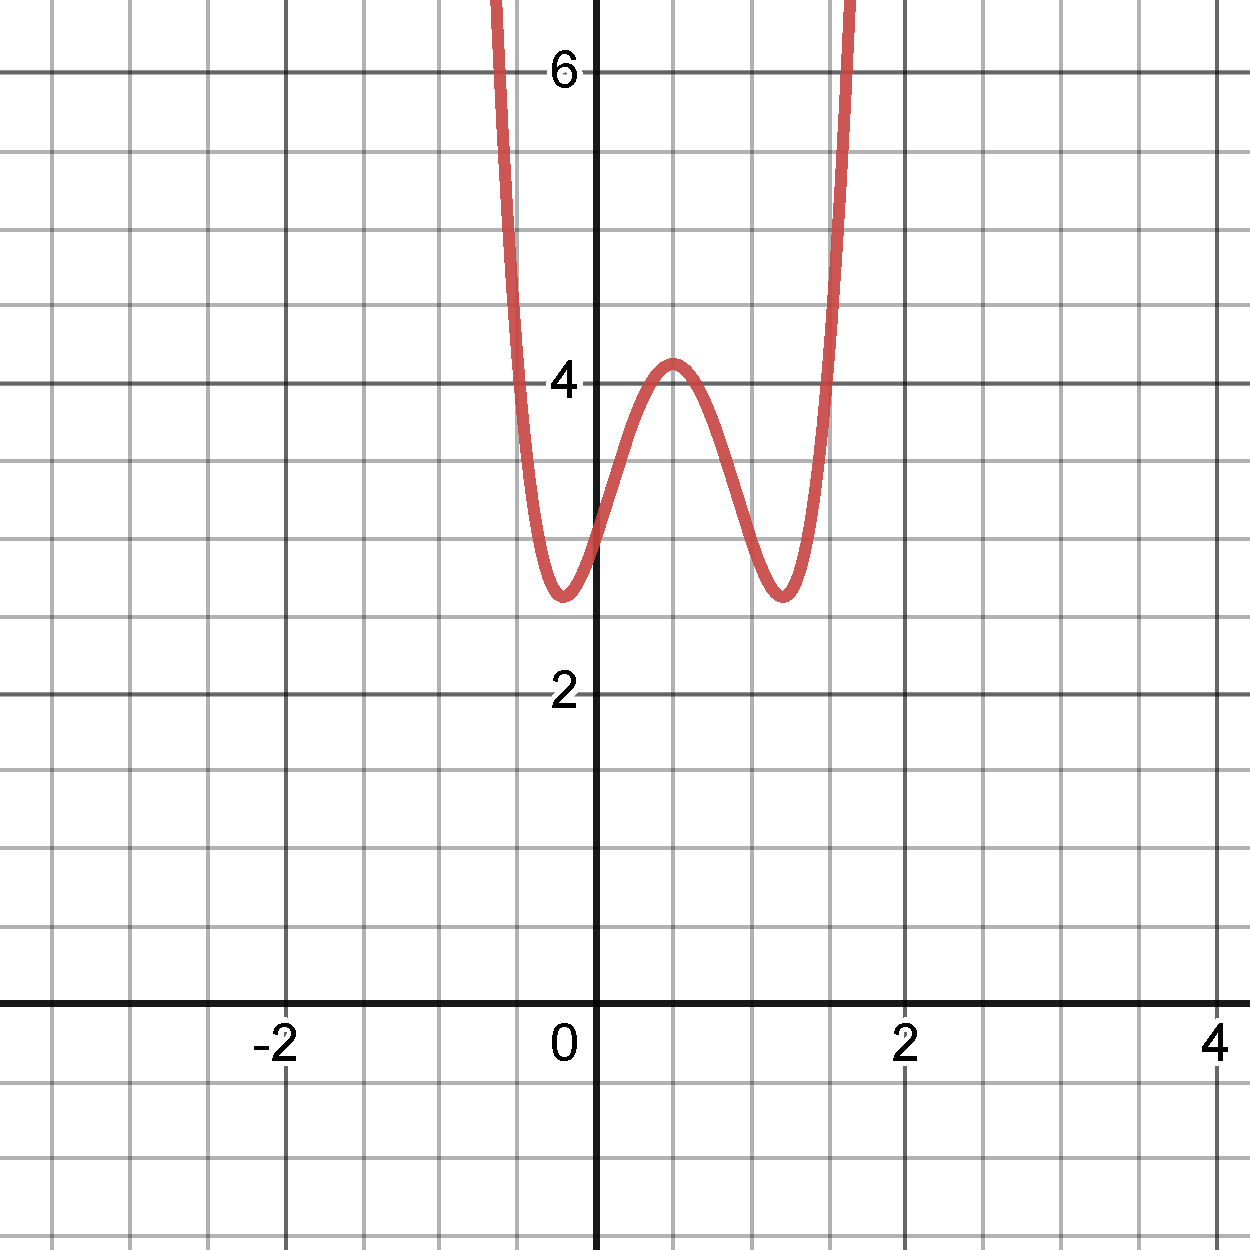
\includegraphics[clip, trim=2cm 2cm 1cm 3cm, height=0.5\textheight]{images/esperance.pdf}
	\end{center}
\end{frame}
\begin{frame}{Au-dessus de l'intervalle $[0,1]$}
Ici, la fonction $f(p)$ correspond à l'espérance de la variable aléatoire $X$ selon la valeur du paramètre $p$ choisi.
\begin{center}
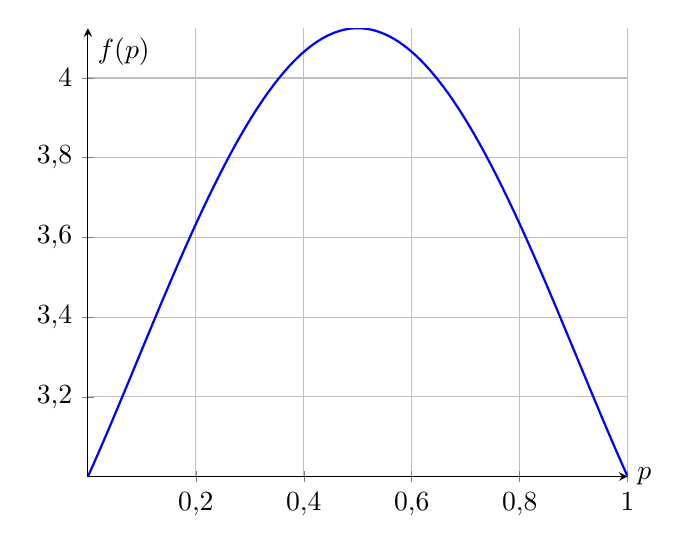
\begin{tikzpicture}
    \begin{axis}[
        axis lines = middle,
        xlabel = $p$,
        xlabel style = {at={(1,0)}, right},  % Place l'étiquette à droite
        ylabel = {$f(p)$},
        samples = 100,
        domain = 0:1,
        grid = major,
        restrict y to domain=-10:10
    ]
        \addplot[blue, thick] {3 + 3*x + 3*x^2 - 12*x^3 + 6*x^4};
    \end{axis}
\end{tikzpicture}
\end{center}
\end{frame}
\begin{frame}{Optimisation de l'espérance}
	\small
	Pour trouver les valeurs de $p$ qui maximise ou minimise l'espérance, on doit optimiser la fonction
	\[f(p)=3 + 3 p + 3 p^2 - 12 p^3 + 6 p^4\]
	sous la contrainte que $p\in\interval{0}{1}$.\pause~ On trouve que la dérivée de $f$ s'annule en $p=1/2$ et en $p=1/2\pm \sqrt{2}/2$. La valeur critique $p=1/2$ correspond à un maximum relatif, alors que les deux autres valeurs sont à l'extérieur du domaine considéré. La frontière du domaine comprend $2$ éléments, à savoir $p=0$ et $p=1$. On constate qu'en ces points, l'espérance est minimale (valeur de $3$).
	
	On en déduit que si les deux équipes sont de même calibre, l'espérance du nombre de parties nécessaires pour déterminer un vainqueur est $f(1/2)=33/8=\num{4,125}.$ Dans le cas d'une série $4$ de $7$, ce nombre grimpe à $\num{5,8125}$.
\end{frame}
\begin{frame}{La loi de Poisson}
	\begin{defn}
		La \defi{loi de Poisson} de paramètre $\nu$, est une distribution de probabilité dont la fonction de masse est donnée par
		\[
		\P{X=k}=\begin{cases} \mathlarger{\frac{e^{-\nu}\nu^k}{k!}} &\text{si}~k\in\N,\\
			0 & \text{sinon}
			.\end{cases}
		\]
		On écrit alors que
		\[X\sim \loiPoisson{\nu}.\]
	\end{defn}
\end{frame}
\begin{frame}[t]{L'espérance d'une v.a. de loi $\loiPoisson{\nu}$}
	\begin{prop}
		L'espérance d'une v.a. suivant une loi de Poisson de paramètre $\nu$ est $\nu$.
	\end{prop}
\end{frame}
\begin{frame}{La loi de Poisson comme cas limite de la binomiale}
	Dans un exemple précédent, la moyenne du nombre de bonbons rejetés par le contrôle de la qualité pour une journée est de $10$. Calculons la probabilité qu'une v.a. suivant une loi de Poisson de paramètre $10$ prennent des valeurs entre $0$ et $4$. Cela correspond à :
	\[\frac{e^{-10}10^0}{0!}+\frac{e^{-10}10^1}{1!}+\frac{e^{-10}10^2}{2!}+\frac{e^{-10}10^3}{3!}+\frac{e^{-10}10^4}{4!}\approx\num{0.02925269}.\]
\end{frame}
\begin{frame}{La loi de Poisson comme cas limite de la binomiale --- suite}
	Soit $X$ une v.a. suivant une loi binomiale de paramètres $n$ et $p$. Nous allons supposer que $n$ est grand et $p$ petit. C'était le cas dans l'exemple de l'usine de bonbons.\pause
	
	Fixons une valeur de $\nu>0$. Pour chaque entier $n>\nu$, le nombre $p_n=\frac{\nu}{n}$ est un nombre dans l'intervalle $\interval[open]{0}{1}$. Pour chacune de ces valeurs de $n$, on peut considérer une v.a. $X_n$ dont la loi est une binomiale de paramètres $n$ et $p_n$. La fonction de masse de $X_n$ est donnée par
	\[
	\P{X_n=k}=\begin{cases} 
		\binom{n}{k}\left(\frac{\nu}{n}\right)^k\left(1-\frac{\nu}{n}\right)^{n-k} &\text{si}~k\in\{0,1,2,\ldots, n\},\\
		0 & \text{sinon}.
	\end{cases}
	\]
\end{frame}
\begin{frame}{Passage à la limite}
	Pour $k\in\{0,1,2,\ldots, n\}$, nous avons que
	\begin{align*}
		\lim_{n\rightarrow\infty}\P{X_n=k}&=\lim_{n\rightarrow\infty}\frac{n!}{k!(n-k)!}\frac{\nu^k}{n^k}\left(1-\frac{\nu}{n}\right)^{n-k}\\
		&=\frac{\nu^k}{k!}\lim_{n\rightarrow\infty}\frac{n!}{(n-k)!n^k}\left(1-\frac{\nu}{n}\right)^{n}\left(1-\frac{\nu}{n}\right)^{-k}\\
		&=\frac{\nu^k}{k!}\underbrace{\lim_{n\rightarrow\infty}\frac{n!}{(n-k)!n^k}}_{=1}\underbrace{\lim_{n\rightarrow\infty}\left(1-\frac{\nu}{n}\right)^{n}}_{=e^{-\nu}}\underbrace{\lim_{n\rightarrow\infty}\left(1-\frac{\nu}{n}\right)^{-k}}_{=1}\\
		&=\frac{e^{-\nu}\nu^k}{k!}.
	\end{align*}
\end{frame}
\begin{frame}{La loi hypergéométrique}
	Une urne contient $N$ boules gagnantes et $M$ boules perdantes. On tire $n$ boules au hasard. On définit $X$ la v.a. correspondant au nombre de boules gagnantes pigées.
	\vfill
	\pause
	\textbf{Cas 1 : le tirage se fait avec remise}
	
	Dans ce cas, $X\sim \loibinomiale{n}{\frac{N}{N+M}}$.\\
	\vfill
	\pause
	\textbf{Cas 2 : le tirage se fait sans remise}
	Une urne contient $N$ boules gagnantes et $M$ boules perdantes. On tire $n$ boules au hasard. On définit $X$ la v.a. correspondant au nombre de boules gagnantes pigées.
	Quelle est la distribution de $X$?
	\vfill
\end{frame}
\begin{frame}
\begin{defn}
Une urne contient $N$ boules gagnantes et $M$ boules perdantes. On tire $n$ boules au hasard. On définit $X$ la v.a. correspondant au nombre de boules gagnantes pigées. On dira que \[X\sim \loihypergeometrique{n}{N}{M},\]
où
\[
p_X(k)=\begin{cases}
\frac{\binom{N}{k}\binom{M}{n-k}}{\binom{N+M}{n}}&\text{si $k\in\N$,}\\
0&\text{sinon.}
\end{cases}\]
\end{defn}
\end{frame}
\begin{frame}[allowframebreaks]{Bibliographie}
\printbibliography[heading=none]
\vspace{0.5cm}

 \begin{rems}
 	\begin{itemize}
 		\item Ce document est rédigé avec Beamer, une classe de \LaTeX.
		\item La formulation des définitions et énoncés est fortement inspirée de \cite{belisle}.
 	\end{itemize}
 \end{rems}

 	\vfill
 	\footnotesize Pour signaler une erreur dans ce document, veuillez écrire à~\href{mailto:jerome.soucy@mat.ulaval.ca}{jerome.soucy@mat.ulaval.ca}.
 \end{frame}
\end{document}